\chapter{Integrazione}

L'architettura dove avrei dovuto lavorare è formata da uno stack classico con spring che si occupa del lato backend e angularjs che invece gestisce il livello frontend, tutta la codebase viene versionata usando Subversion. Subversion è un version control system di tipo centralizzato, questo significa che si ha un server centrale che contiene tutto il codice. Il problema di usare un versionamento di questo tipo è che per poter sviluppare codice si deve essere collegati al server remoto altrimenti non è possibile apportare modifiche.
\begin{figure}[H]
    \centering
    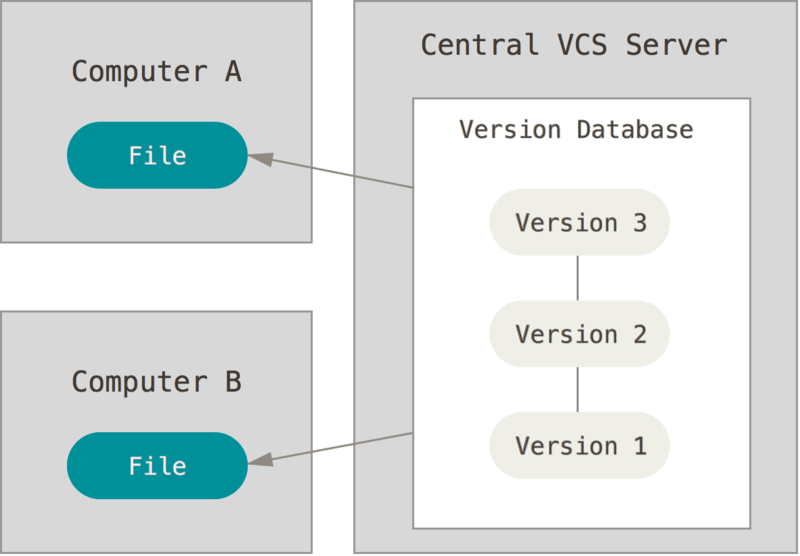
\includegraphics[width=0.6\textwidth]{img/centralized.png}
    \caption{Centralized Version Control System}
\end{figure}
Alcune dipendenze lato frontend non possono essere usate, come socket.io, oppure non servono più, come express perchè il sistema in cui andiamo ad aggiungere questo modulo già prevede la creazione di uno web server. Per quanto riguarda socket.io ho dovuto riscrivere il codice andando a sostituire la libreria con \textbf{angular-socket-io}, un porting sotto forma di componente angularjs in modo da poter ricreare lo scambio di messaggi instaurato nel prototipo.
Il modulo è risultato essere composto da 3 elementi: 
\begin{itemize}
  \item \textbf{chatbot.html} la versione minimale dell'interfaccia web del prototipo,
  \item \textbf{chatbotUtilityService.js} script di utility in cui vengono definite le funzioni per comunicare con il server rasa,
  \item \textbf{chatbotController.js} la cui responsabilità è quella di gestire la comunicazione con il server rasa e modificare l'interfaccia grafica con la risposta
\end{itemize}
Il motivo per cui l'interfaccia è stata creata minimale è che per poter applicare una modifica grafica sono necessari degli studi di user experience per capire come renderla il più facile possibile da usare per l'utente. Considerando che la web app può essere visualizzata da tantissimi dispositivi diversi come cellulari di diversa forma o tablet e anche computer, il lavoro è stato demandato al reparto specializzato che avrebbe poi stabilito come questa sarebbe dovuta essere fatta.
Lo script di utility è stato creato per estrarre dal controller molte delle responsabilità che aveva, in modo tale da rendere più snella la leggibilità dei componenti e più facile la manutenzione. In questo componente si possono trovare tutte le funzioni che sono necessarie per la comunicazione in entrata e uscita verso il server dove si trova l'intelligenza artificiale.
Per poter utilizzare in produzione l'intelligenza artificiale è stato creato un server linux dedicato con tutte le dipendenze necessarie ad eseguire le fasi di preparazione e running di Rasa. Questo permette di rimuovere la complessità di creazione di nuovi modelli nella macchina locale di sviluppo rendendo più agile il lavoro di manutenzione e aggiornamento delle nuove versioni.
\begin{figure}[H]
 \centering
  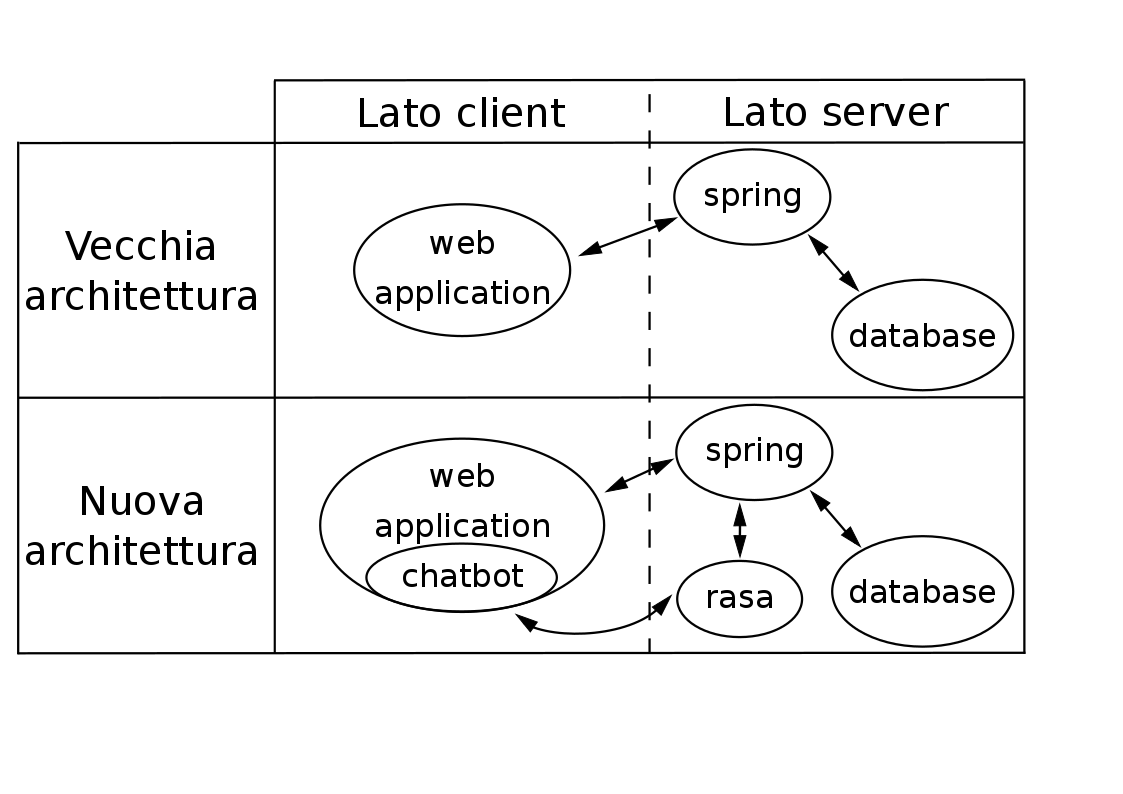
\includegraphics[width=0.6\textwidth]{img/old-new.png}
 \caption{Vecchia e nuova architettura}
\end{figure}
Rimane comunque il problema del dataset con cui viene generato il modello dell'intelligenza artificiale, come è stato già detto, più stories abbiamo e più l'intelligenza è migliore. Ci sono due modi per creare nuove conversazioni: rilasciare una versione beta della chat in modo da ottenere molte conversazioni reali, oppure creare un team aziendale che rimpiazza il cliente inserendo quante più conversazioni differenti possibili.
Questa prima versione del chatbot ha la capacità esclusiva di listare i conti correnti di un cliente ed eseguire dei pagamenti preimpostati, la scelta di limitare le funzionalità è dovuta ad un fatto di sicurezza perchè ancora i modelli generati non erano abbastanza sicuri da poter essere usati in ambiente di produzione.
